\chapter{Introdução}
  
  	A aviação é o principal meio de transporte capaz atravessar grandes distâncias, a sua utilização é fundamental para o crescimento das empresas e também para o desenvolvimento do turismo mundial. O transporte aéreo é um serviço que oferece beneficios de ordem social e de ordem econômica. Por ser utilizado no turismo e no comercio, ele contribui para o crescimento da economia mundial e é essencial para o rápido transporte de pessoas e de mercadorias ao redor do mundo. Finalmente, o transporte aéreo melhora a qualidade de vida das pessoas proporcionando lazer e experiências com outras culturas.
  	
  	O uso da aviação comercial tem crescido significativamente nas últimas décadas. Esse rápido crescimento pode ser atribuído a um grande número de fatores. Primeiro, o aumento da renda e da qualidade de vida em muitas partes do mundo tem incentivado as pessoas a viajar para outras áreas e explorar novas oportunidades. Segundo, a demanda tem aumentado junto com a confiança na aviação como um meio seguro de viajar. Terceiro, o aumento da eficiência nas operações tem acirrado a competitividade e reduzido as taxas e os custos das passagens. Finalmente a globalização tem forçado a viagem de pessoas para fazer negócios em outros país e também para aperfeiçoar as relações políticas e sociais. Espera-se que os impactos desses fatores continuem a acontecer porém com intensidades diferentes.
  	
  	O aumento do numero de companhias aéreas tem aumentado a necessidade de obtenção de melhores benefícios, redução dos custos e aumento das receitas. Porém os problemas presentes na indústria aeronáutica são complexos envolvendo múltiplas decisões conflitantes que precisam ser otimizadas de uma só vez. Diversas técnicas são desenvolvidas e usadas para tentar melhorar o planejamento e a operação das empresas aéreas. Muitas dessas técnicas estão disponíveis na literatura e científica nos campos da pesquisa operacional e da matemática e normalmente são modelados para funcionar em sistemas computadorizados de alta capacidade com a finalidade de automatizar, ou pelo menos auxiliar, a tomada de decisões. Essas técnicas se tornam mais necessárias a medida que a empresa aérea cresce e a tomada de decisão, baseada nos julgamentos individuais e nas experiências, se tornam mais difíceis \cite{ahmed2009}. A seguir alguns dos principais problemas presentes na indústria aeronáutica são detalhados.
  	
    A indústria aeronáutica apresenta uma grande quantidade de problemas inter conectados, o que torna esse campo de pesquisa bastante interessante para a pesquisa operacional. Esses problemas apresentam um alto grau de complexidade e a maioria possui uma natureza combinatória explosiva. Pode-se dizer que o problema inicial é a modelagem de mercado, que planeja os voos de cada regiao baseado na demanda. A atribuição da frota define qual o tipo de aeronave que irá atender cada um dos voos planejados. A construção de trilhos de aeronaves define o sequenciamento dos voos a partir do um conjunto de voos que tenha sido atribuído a um tipo de aeronave. A construção de dias de trabalho, parte dos trilhos gerados e define as subsequências que poderão ser operados por uma tripulação. E a criação das escalas dos tripulantes que define qual será a jornada de trabalho dos tripulantes.
    
    Por causa da dificuldade que é inerente a essa classe de problemas a qualidade das soluções obtidas manualmente são muito aquém da melhor solução possível. 
  
Nos dias de hoje, no entanto, com o avanço da tecnologia e o aumento da competitividade desenvolver soluções com melhor qualidade acaba se tornando um fator decisivo para a permanência no mercado, tornando-se então necessário a obtenção de soluções de forma mais rápida, mais barata e utilizando menos recursos. Outra  característica que reforça a necessidade da obtenção de melhores soluções é o aumento do tamanho e da complexidade das instâncias trabalhadas. A partir desse cenário pode-se perceber a necessidade de utilização de técnicas de otimização, na literatura tem se observado um crescimento no número de trabalhos que se utilizam de metaheurísticas como método de resolução.
  
As metaheurísticas podem ser definidas como um conjunto de procedimentos de caráter geral, com capacidade de guiar o procedimento de busca, tornando-o capaz de escapar de ótimos locais. Elas têm como objetivo, encontrar uma solução tão próxima quanto possível da solução ótima do problema com baixo esforço computacional.
  
Em geral, as metaheurísticas são bastante utilizadas na resolução de problemas de otimização. Esses problemas, também conhecidos como problemas NP-difíceis\abbrev{NP}{Non-Polinomial}, podem ser definidos como um conjunto de problemas para os quais ainda não existe um algoritmo que os resolvam de forma exata e em tempo polinomial \citep{maritan}.
  
Para esses tipos de problemas o uso de métodos exatos é bastante restrito, uma vez que o esforço computacional para encontrar uma solução exata em instâncias reais é consideravelmente alto. No entanto, na prática, é suficiente encontrar uma solução próxima do ótimo global. 

A literatura pesquisada mostra uma grande quantidade de tentativas de resolver o problema utilizando modelagens matemáticas, que apesar de garantir a solução ótima não se mostra viável para resolver grandes instâncias. \citep{clarke97}. Alguns trabalhos mostram a similaridade desse problema com o problema do caixeiro viajante assimétrico \cite{clarke97}. E outros resolvem uma parte do problema utilizando metaheurísticas.\citep{arguelo1007}
%#############################################
%{\large >>>> Descrever em que tem se baseado a solução desse problema na literatura <<<<}
%#############################################

Os principais problemas relacionados dizem respeito ao planejamento envolvendo a criação de linhas de trabalho tanto para as aeronaves quanto para a tripulação. O objetivo costuma ser a minimização dos custos operacionais ou a maximização dos rendimentos. Custos operacionais consiste nos custos envolvidos com combustíveis, óleo, taxas de aterrissagem e a perda de rendimentos com a utilização de aeronaves com menos assentos do que a demanda de passageiros, porém fatores como bem estar dos passageiros também podem ser levados em consideração.

	Os problemas de planejamento que envolvem as aeronaves mais estudados na literatura são o Fleet Assigment e o Aircraft Rotation. E os que envolvem a tripulação são conhecidos como Crew Pairing e o Crew Scheduling.

	O problema Fleet Assigment trata da alocação da frota, ou seja, é determinado o tipo de equipamento a ser utilizado em cada voo [Pimentel, 2005]. O problema Aircraft Rotation será descrito mais adiante. O problema Crew Pairing visa obter o melhor conjunto de pairings \footnote{Pairing é o conjunto de voos que pode ser guiados por uma tripulação sem que seja violadas quaisquer regras da legislação vigente e que ao final do ultimo voo o tripulante esteja de volta a sua cidade base. }  tal que cada voo seja coberto por pelo menos um pairing. Gastos com alojamentos, alimentação, transporte em terra e deadheads \footnote{Deadhead é o voo que o tripulante viaja sem trabalhara com a finalidade de transporte para outra localidade normalmente para sua base ou para suprir uma nova demanda. } devem ser levados em consideração. O problema Crew Scheduling tem o objetivo de atribuir os pairings a tripulação disponível na companhia aérea, acrescentando as atividades de solo tais como call \footnote{Call é o tempo que a tripulação tem para se apresentar a companhia aérea antes de iniciar de fato seu turno de trabalho.} , Stand-by duties \footnote{Stand-by duties são turnos em que o tripulante fica a disposição da companhia aérea afim de suprir possíveis eventualidades.}  e dias de descanso. O objetivo dessa etapa é fazer uma distribuição da forma mais justa possível, tentando balancear a quantidade de trabalho (horas a serem voadas) entre os tripulantes, e também tentar cumprir todas as solicitações da tripulação em relação a preferência dos dias de descanso e das tarefas a serem realizadas.

	Após as designação da frota de aeronaves ao conjunto de voos existentes segue-se o problema de construção de trilhos de aeronaves (PCTA) \abbrev{PCTA}{Problema de Construção de Trilhos de Aeronaves} que também é conhecido na literatura como Aircraft Rotation Problem (ARP) \abbrev{ARP}{Aircraft Rotation Problem}. O PCTA é um dos principais problemas presentes na industria da aviação. No PCTA o objetivo é a construção, para cada uma das frotas da companhia (e para os voos a elas alocados), de sequências encadeadas de vôos que possam ser operados por uma única aeronave \citep{abiliolivro}. Cada uma dessas sequências recebe o nome de trilho.
 
	O sequenciamento dos voos pode ocorrer de 4 formas distintas aqui denominado de arcos. Os arcos do tipo 1 permitem a ligação de voos sem a utilização de atrasos e/ou reposicionamentos. Os arcos do tipo 2 utilizam atrasos mas não o reposicionamento. Os arcos do tipo 3 permitem o sequenciamento com a utilização de um voo de reposicionamento mas sem inserir atraso em nenhum dos voos envolvidos. Os arcos do tipo 4 utilizam-se de atrasos e de um voo de reposicionamento para fazer a ligação entre dois voos.
 
	Para resolver o PCTA, devemos estar cientes de algumas restrições que envolvem tempo e espaço. Por exemplo, um avião não pode partir antes da chegada do vôo que lhe antecede, nem de um local diferente da cidade de destino deste mesmo vôo. Há também a restrição de que um vôo deve permanecer em solo, entre conexões, por um período de tempo que seja suficiente para fazer a troca de passageiros e abastecimento da aeronave e quando for o caso para a troca de tripulação, esse tempo varia de acordo com o aeroporto. O PCTA sofre um grande quantidade de restrições sendo as mais importantes as temporais e geográficas.
 
	Vale ressaltar que na resolução do PCTA deve-se levar em consideração as particularidades especificas de cada companhia aérea como o número de aviões disponíveis na frota, o atraso máximo permitido nos voos, a quantidade máxima de voos que podem sofrer atraso, o número máximo de voos que podem ser cancelados, o número máximo de voos de reposicionamento que podem ser criados entre outros.
 
	Outro aspecto importante diz respeito às restrições de manutenção. Sabe-se que um avião deve ter checagens periódicas. Oportunidades de realizar essas tarefas ocorrem apenas em algumas conexões potencialmente disponíveis. Como consequência, uma sequência de voos deve ser construída de forma que essas restrições não sejam violadas. A fim de incorporar essas restrições facilmente ao nosso framework, assumimos que as rotações são designadas a tipos não específicos de aeronave. Dessa forma, se uma aeronave tem necessidade de manutenção, um vôo especial é criado com origem e destino na base de manutenção escolhida. O tempo desse vôo é exatamente o tempo de manutenção [Pontes, 2003].
 
	De uma maneira geral, o principal objetivo do PCTA é a minimização do número de trilhos seguido da minimização do custo total dos trilhos gerados. Esse custo pode envolver diversos componentes, sendo o tempo médio diário de utilização das aeronaves um dos mais importantes \citep{abiliolivro}.
 
	Abaixo na Figura \ref{arpexample} temos dois exemplos de montagem de trilhos feitas a partir de um conjunto fictícios de voos. Cada caixinha laranja e azul representa um voo, onde a parte laranja representa o tempo de solo que cada voo deve obedecer e a azul seria o tempo de voo da cidade de origem para a cidade de destino. As letras A, B, C, D, E representam as cidades e a linha pontilhada indica o tempo de inicio e de termino de cada voo.

\begin{figure}[ht]
	\centering
	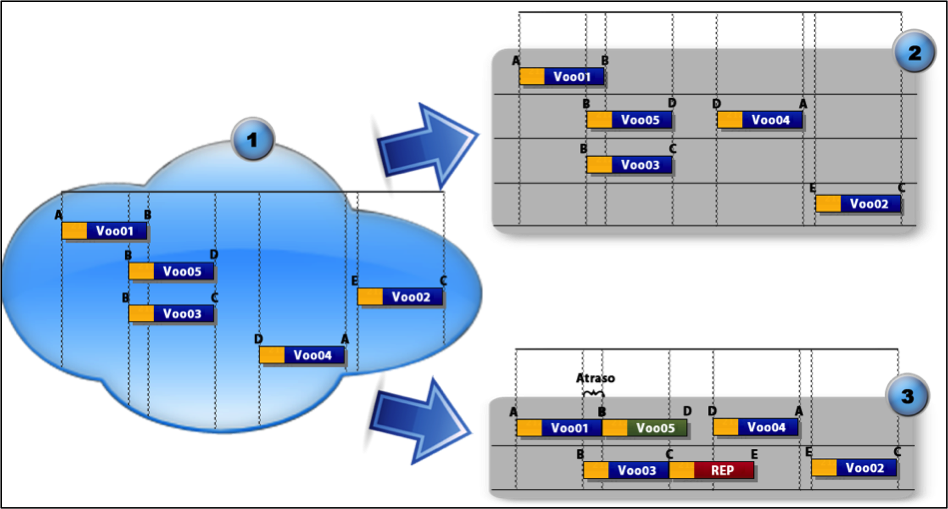
\includegraphics[scale=0.9]{./img/arpexample}
	\caption{Construção de Trilhos de Aeronaves}
	\label{arpexample}
\end{figure}

A parte 1 da Figura \ref{arpexample} representa os voos da companhia que ainda não foram cobertos por nenhuma aeronave e nas partes 2 e 3 são demonstrado duas formas de organizar esses voos em trilhos. 

	Na parte 2 temos a melhor forma possível de se organizar os voos da parte 1 utilizando apenas os arcos do tipo 1, ou seja sem a utilização de atrasos ou de voos de reposicionamento. Dessa forma se consegue uma formação com 4 trilhos.

	Na parte 3 temos a melhor forma de organizar os voos utilizando todos os arcos e um atraso máximo equivalente a um tempo de solo. Dessa forma se consegue uma formação com apenas 2 trilhos.

	Pode-se verificar que a utilização de diferentes tipos de arcos pode proporcionar uma melhora significativa  no número de trilhos. Porém essa abordagem faz com que o número de soluções possíveis tenha uma cardinalidade muito superior a utilização de arcos apenas do tipo 1 que por si só já gera uma quantidade de soluções bem elevada, por isso os arcos devem ser utilizados de forma controlada. 

	Nesse trabalho propomos o desenvolvimento de um método híbrido baseados em metaheurísticas e em programação para resolução do PCTA. O método proposto procura combinar a eficiência computacional das metaheurísticas com a rápida convergência dos métodos exatos. Além disso ficou constatado pelo levantamento da literatura acerca do PCTA que se tem uma falta de instâncias sobre o problema que permitam uma melhor comparação dos resultados obtidos, logo também propomos um conjunto de instância baseado em uma instância real da TAM, com vários tamanhos e complexidades. 

%#############################################
{\large	>>>> Fazer uma breve descrição de programação linear, maiores detalhes serão dados na fundamentação teórica. <<<<	}
%#############################################

\section {Objetivos do trabalho}

Tendo em vista os aspectos apresentados, o objetivo principal dessa proposta de trabalho consiste no desenvolvimento de um método híbrido baseado em metaheurísticas e programação linear para a resolução do problema construção de trilhos de aeronaves (PCTA). O método proposto irá se basear em uma metaheurísticas, afim de explorar a eficiência computacional, e irá ser combinada com etapas de refinamentos composta por métodos exatos para acelerar a convergência e adicionalmente fugir de mínimos locais.

Além disso irá ser proposto um conjunto de instâncias baseados em uma instância real da TAM variando em complexidade e tamanho, essas instâncias irão permitir uma melhor comparação desse trabalho com outros.

\section {Organização da proposta }

A dissertação está estruturada da seguinte forma:

\begin{itemize}

\item Capítulo 1: Apresenta a motivação e as vantagens de resolver o PCTA utilizando metaheurísticas e programação linear e enfatiza a importância desse problema na indústria aeronáutica.  Ao final os objetivos do trabalho são descritos.

\item Capítulo 2: Apresenta a fundamentação sobre a otimização, metaheurísticas e programação linear. Na seção referente à otimização além da descrição serão discutidos algumas heurísticas  construtivas e de refinamento. A seção referente às metaheurísticas irá iniciar com uma descrição seguida pela descrição das metaheurísticas utilizadas no trabalho, como o Greedy Randomized Adaptive Search Procedure (GRASP) e o Iterated Local Search (ILS). E a seção referente a programação linear vai descrever como o algoritmo simplex consegue resolver problemas modelados matematicamente. Ao final da fundamentação teórica será feita uma revisão dos principais trabalhos descritos na literatura relacionada ao presente trabalho.

\item Capítulo 3: Mostra como foi obtida a malha da companhia de transporte aéreo TAM e como foi gerado as instâncias que são utilizadas no trabalho.

\item Capítulo 4: Descreve o método proposto nesse trabalho, os parâmetros, as restrições e a modelagem matemática utilizada.

\item Capítulo 5: Apresenta alguns resultados preliminares que já foram obtidos com o método que é utilizado atualmente.

\item Capítulo 6: Apresenta as referencias bibliográficas que deram suporte a confecção do presente trabalho.

\item No final é apresentado o cronograma de trabalho proposto durante os 24 meses de mestrado. 
\end{itemize}